\documentclass{article}

\newcommand{\coursename}{Bayesian Statistics}
\newcommand{\coursecode}{052499}
\newcommand{\coursesupervisor}{Alessandro Colombi}
\newcommand{\courseprof}{Prof. A. Guglielmi}
\newcommand{\papertitle}{Stochastic Block Model Prior with Ordering Constraints for Gaussian Graphical Models}

\usepackage[british]{babel} % british per avere l'access date nella bibliografia come i comuni mortali
\usepackage[utf8]{inputenc}
\usepackage[margin=1.5in]{geometry}
\usepackage{amsmath,amsthm,amsfonts,amssymb}
\usepackage{lipsum}
\usepackage{bm,bbm}

\usepackage{booktabs}
\usepackage{multirow}
\usepackage{xcolor}
\usepackage{colortbl}

\usepackage{multicol}
\usepackage[none]{hyphenat}
\usepackage[small]{titlesec}
\usepackage{minted}
\usemintedstyle{default} % https://pygments.org/styles/

% Bibliography
\usepackage{csquotes}% Recommended
\usepackage[
    style=authoryear,
    url=true,
    sorting=none,
    natbib
    ]{biblatex}
\addbibresource{../bibliography.bib}% Syntax for version >= 1.2
% use \cite or \parencite

\usepackage{import}
\usepackage{pdfpages}
\usepackage{transparent}
\usepackage{xcolor}
\usepackage{graphicx}
\graphicspath{ {./images/} } % Path relative to the main .tex file
\usepackage{float}
\usepackage[font=footnotesize]{caption}
\usepackage{booktabs}

\usepackage{fontawesome}
\usepackage{authblk}

\usepackage{bookmark}% loads hyperref too
    \hypersetup{
        %pdftitle={Fundamentos de C\'alculo},
        %pdfsubject={C\'alculo diferencial},
        bookmarksnumbered=true,
        bookmarksopen=true,
        bookmarksopenlevel=1,
        hidelinks,% remove border and color
        pdfstartview=Fit, % Fits the page to the window.
        pdfpagemode=UseOutlines, %Determines how the file is opening in Acrobat; the possibilities are UseNone, UseThumbs (show thumbnails), UseOutlines (show bookmarks), FullScreen, UseOC (PDF 1.5), and UseAttachments (PDF 1.6). If no mode if explicitly chosen, but the bookmarks option is set, UseOutlines is used.
    }

\setlength{\marginparwidth}{3.4cm}

%#########################################################

\title{
    \begin{figure}[htpb]
        \centering
        
\includegraphics[scale=0.2]{images/logo-polimi}
    \end{figure}
    \normalfont \normalsize 
    \textsc{MSc. in Mathematical Engineering A.Y. 2022/2023\\ 
    Project Report of \coursename\ (\coursecode) -- \courseprof \\
    Supervisor: \coursesupervisor} \\
    [10pt] 
    \rule{\linewidth}{0.5pt} \\ [6pt] 
    \huge \papertitle \\
    \rule{\linewidth}{2pt}  \\ [10pt]
}

%\author{Teo Bucci, Filippo Cipriani, Filippo Pagella,\\ Flavia Petruso, Andrea Puricelli, Giulio Venturini}
%\author{T. Bucci, F. Cipriani, F. Pagella,\\ F. Petruso, A. Puricelli, G. Venturini}
%\author{T. Bucci\footnote{teo.bucci@mail.polimi.it, 10621873}, F. Cipriani\footnote{filippo.cipriani@mail.polimi.it, 10596877}, F. Pagella\footnote{filippo.pagella@mail.polimi.it, 10616351},\\ F. Petruso\footnote{flavia.petruso@mail.polimi.it, 10544566}, A. Puricelli\footnote{andrea3.puricelli@mail.polimi.it, 10632135}, G. Venturini\footnote{giulio.venturini@mail.polimi.it, 10624098}}

%\affil{\texttt{\{teo.bucci, filippo.cipriani, filippo.pagella, flavia.petruso, andrea3.puricelli, giulio.venturini\}@mail.polimi.it}}

\makeatletter
\renewcommand\AB@affilsepx{, \protect\Affilfont}
\makeatother
\author[1]{Teo Bucci}
\author[2]{Filippo Cipriani}
\author[3]{Filippo Pagella}
\author[4]{Flavia Petruso}
\author[5]{Andrea Puricelli}
\author[6]{Giulio Venturini}
\affil[1]{10621873}
\affil[2]{10596877}
\affil[3]{10616351}
\affil[4]{10544566}
\affil[5]{10632135}
\affil[6]{10624098}

\date{\normalsize \today}

\begin{document}

\maketitle

\begin{abstract} %in progress - per ora non lo manderei
Gaussian graphical models are used to study the conditional dependence structure among variables through the presence or absence of edges in the underlying undirected graph. In many applications, the variables can be grouped so that the graph to be learnt from the data has a block structure. Stochastic block models offer a powerful tool to detect such structure in a network. The goal of this project is to propose a new flexible prior that accounts for a random partition of the nodes, respects their ordering constraints and allows to learn a block-structured graph.

\vspace*{0.5cm}

\begin{center}
    The source code of the entire project,\\
    including this report and the presentations, is available at\\
    \faGithub\ \url{https://github.com/teobucci/bayesian-statistics-project}
\end{center}
\end{abstract}

\clearpage

\tableofcontents

%\setlength{\columnsep}{0.8cm}
%\begin{multicols}{2}
    %!TEX root = ./main.tex

\section{The model}

\begin{frame}{Our model}

\alert{Goal}: given a set of $n$ data with $p$ variables, simultaneously infer the conditional dependence structure of such variables and their clustering.

\pause

\alert{Constraint}: the partition must respect the original order of the variables.

\pause

\begin{align*}
    \bm{y}_1, \ldots, \bm{y}_n \mid \bm{K} & \iid \mathcal{N}_p(\mathbf{0}, \bm{K}^{-1} ) \\
    \bm{K} \mid G & \sim \GWish(b, D)\\
    P((i,j)&\in E\mid \bm{z},Q) = Q_{z_{i} z_{j}},\,\text{independent}\\
        Q_{rs} \mid \bm{z} &\ind \Beta(a,b), 1\leq r\leq s\leq M\\
    \rho & \sim f_{\rho} \left(\rho\right)
\end{align*}
% Attenti ai parametri della Beta, ho visto che ogni tanto avete messo a,b e ogni tanto \alpha,\beta. TODO

Notation for the partition: $\rho$ vector of cardinalities, $\bm{z}$ vector of groups memberships.

\end{frame}

\begin{frame}

$Q$ is marginalized out.

% chi è f_G e S_uv, T_uv % TODO
% la prior sulla partizione è quella di Martinez e Mena % TODO

\end{frame}

\section{The sampling strategy}

\subsection{Overview of the sampling strategy}

\begin{frame}{Block Gibbs Sampler}
    Conditional distributions for our model:
    
    \begin{table}[tb]
        \centering
        \begin{tabular}{ll}
        \toprule
        Graph and Precision & $\small P(\bm{K},G \mid \bm{Y},\bm{z}) \propto P(\bm{Y} \mid \bm{K})P(\bm{K} \mid {G}) P(G \mid \bm{z})$ \\
        \hline
        Random Partition & $\small P(\bm{z} \mid \bm{Y},\bm{K},G) \propto P(\bm{Y} \mid \bm{K})P(\bm{K} \mid {G})P(G \mid \bm{z})P(\bm{z}) \propto P(G \mid \bm{z})P(\bm{z}) $ \\
        \bottomrule
        \end{tabular}
    \end{table}

    \pause 

    We implement a Block Gibbs-Sampler strategy:
    \begin{enumerate}
        \item \alert{Sampling Graph and Precision Matrix}\\
        $G$ and $\bm{K}$ - given $\bm{z}$ - are sampled using a modified version of a Birth-and-Death chain (\cite{mohammadiBayesianStructureLearning2015a}), changing one link at a time.
        \item \alert{Sampling the Random Partition}\\
        Conditionally on $G$, we can sample $\bm{z}$ through an adaptive split and merge\vphantom{changepoint} sampler.
    \end{enumerate}
\end{frame}

\subsection{Updating the graph}

\begin{frame}{Birth and death algorithm for updating the graph}

    \texttt{BDGraph} is an algorithm that follows a Birth-and-Death approach to decide whether to \alert{add} a new edge to the graph or \alert{delete} an already existing one.

    \pause
    
    % https://people.inf.ethz.ch/markusp/teaching/guides/guide-tables.pdf
    \begin{table}[tb]
        \centering
        \begin{tabular}{lcc}
        \toprule
        & Target distribution & B/D rates \\
        \hline
        \textbf{Before} & $P(G,\bm{K} \mid \bm{Y}) \propto \mathcal{L}(\bm{Y} \mid \bm{K})\mathcal{L} (\bm{K} \mid {G})P(G)$ & $\cfrac{P(G')}{P(G)}$ \\
        \textbf{After}  & $P(G,\bm{K} \mid \bm{Y}, \textcolor{sleekRed}{\bm{z}}) \propto \mathcal{L}(\bm{Y} \mid \bm{K})\mathcal{L}(\bm{K} \mid {G})P(G \mid \textcolor{sleekRed}{\bm{z}})$ & $\cfrac{P(G' \mid \textcolor{sleekRed}{\bm{z}})}{P(G \mid \textcolor{sleekRed}{\bm{z}})}$ \\
        \bottomrule
        \end{tabular}
    \end{table}
    where $G' = G^{\pm e}$ and $e$ is an edge.
    \pause
    %We computed the birth and death rates as:
    \[
        \text{Birth rate} \propto \frac{P(G^{+ e}\mid \bm{z})}{P(G\mid \bm{z})} = \frac{S_{uv} + a}{T_{uv} - S_{uv} + b}
        \quad
        \text{Death rate} \propto \frac{P(G^{- e}\mid \bm{z})}{P(G\mid \bm{z})} = \frac{T_{uv} - S_{uv} + b}{S_{uv} + a}
    \]
    \textcolor{red}{TODO: non sappiamo se tenere queste formule dato che S,T,u,v,a,b non sono stati spiegati}
    
\end{frame}

\subsection{Updating the partition}

\begin{frame}{General steps for updating the partition}
    
    We perform an (adaptive) \alert{split and merge}.

    \fg{0.5}{update_partition_splitmerge.pdf}
    \begin{enumerate}
        \item With probability $\alpha_{\text{split}}$, usually $0.5$, choose an \alert{split move}, otherwise a \alert{merge move}. Unless we are forced by extreme cases.
        \begin{enumerate}
            \item Propose a new partition by splitting one group into two or merging two adjacent.
            \item Accept or reject using\vphantom{un banale} Metropolis Hastings. The target is:
            $f(\rho \mid G) \approx f_G(G \mid \rho) f_{\rho}(\rho)$
            \[
                \alpha_{\text{accept}} = \min
                \bigg\{1,
                \overbrace{
                \underbrace{\frac{f_G\left(G \mid \rho'\right)}{f_G(G \mid \rho)}}_{\substack{\text{graph}\\\text{ratio}}}
                \underbrace{\frac{f_\rho\left(\rho'\right)}{f_\rho(\rho)}}_{\substack{\text{partition}\\\text{ratio}}}
                }^{\text{target ratio}}
                \underbrace{\frac{Q(\rho',\rho)}{Q(\rho,\rho')}}_{\substack{\text{proposal}\\\text{ratio}}}
                \bigg\}
            \]
        \end{enumerate}
        
    \end{enumerate}

\end{frame}

\begin{frame}{Shuffle move}
    \begin{enumerate}
        \item[2.] To improve the mixing of the chain we also perform a \alert{shuffle move}.
            \begin{enumerate}
                \item[2.1] Propose a new partition by moving some nodes from a group to an adjacent one.
                \item[2.2] Accept or reject using Metropolis Hastings.
            \end{enumerate}
    \end{enumerate}

    \fg{0.4}{update_partition_shuffle.pdf}
\end{frame}

\begin{frame}{Proposal ratio}

We introduce $\bm{a}^{(t)}$ and $\bm{d}^{(t)}$, two $(p-1)$-dimensional vectors of \alert{weights} to choose the node where to perform the split or the merge. They are unnormalized discrete densities.

\pause

Suppose a split move.

\pause

At each iteration, \alert{draw} node $i$ with probability proportional to $a_{i}^{(t)}$.

\pause

Denoting by $a^{\star} = \sum_{j\in \{\text{admissible split nodes}\}}{a_{j}^{(t)}}$ and $d^{\star} = \sum_{j\in \{\text{admissible merge nodes}\}}{d_{j}^{(t)}}$

\pause

\[
    \frac{Q(\rho',\rho)}{Q(\rho,\rho')}
    =
    \frac{P(\text{choose merge})}{P(\text{choose split})}
    \cdot 
    \frac{P(\text{merge at node $i$})}{P(\text{split at node $i$})}
    =
    \frac{1-\alpha_{\text{split}}}{\alpha_{\text{split}}}
    \cdot
    \frac{\frac{d_{i}^{(t)}}{d^{\star}+d_{i}^{(t)}}}{\frac{a_{i}^{(t)}}{a^{\star}}}
\]
The extreme cases ``every node belonging to the same group'' and ``every node has its own group'' are dealt with separately.

\end{frame}

\begin{frame}{Adaptive step}
    The two weights vectors $\bm{a}^{(t)}$ and $\bm{d}^{(t)}$ are updated at each iteration $t$ as in \cite{bensonAdaptiveMCMCMultiple2018} using the following 
    \textbf{adaptation scheme}.

    \begin{itemize}
        \item If a \alert{split} move at node $i$ has been accepted, then update:
		\[
		\log (a_i^{(t+1)})=\log (a_i^{(t)})+\frac{h}{t/p}(\alpha_{\text{split}}-\alpha_{\text{target}}) .
		\]
        \item If a \alert{merge} move at node $i$ has been accepted, then update:
		\[
		\log (d_i^{(t+1)})=\log (d_i^{(t)})+\frac{h}{t/p}(\alpha_{\text{merge}}-\alpha_{\text{target}}) .
		\]
        \end{itemize}
Where $h>0$ is the initial adaptation, $t/p$ are the iterations $(t)$ per number of nodes $(p)$ and $\alpha_{\text{target}}$ is the target MH acceptance rate.

\end{frame}

\section{Next steps}

\begin{frame}{Next steps}

The first draft of the code is completed.

Next things to do:
    \begin{itemize}
        \item debugging the code
        \item run simulations
        \item perform posterior analysis
    \end{itemize}

\end{frame}

\begin{frame}{Main references}
    % GGM
    \nocite{colombiLearningBlockStructured2022a}
    \nocite{mohammadiBayesianStructureLearning2015a}
    % SBM
    \nocite{legramantiExtendedStochasticBlock2022}
    % Changepoint
    \nocite{bensonAdaptiveMCMCMultiple2018}
    \nocite{martinezNonparametricChangePoint2014}
    
    \printbibliography
    \renewcommand*{\bibfont}{\small}
\end{frame}

\begin{frame}[plain]
    % Add background to content page
    \AddToShipoutPictureFG*{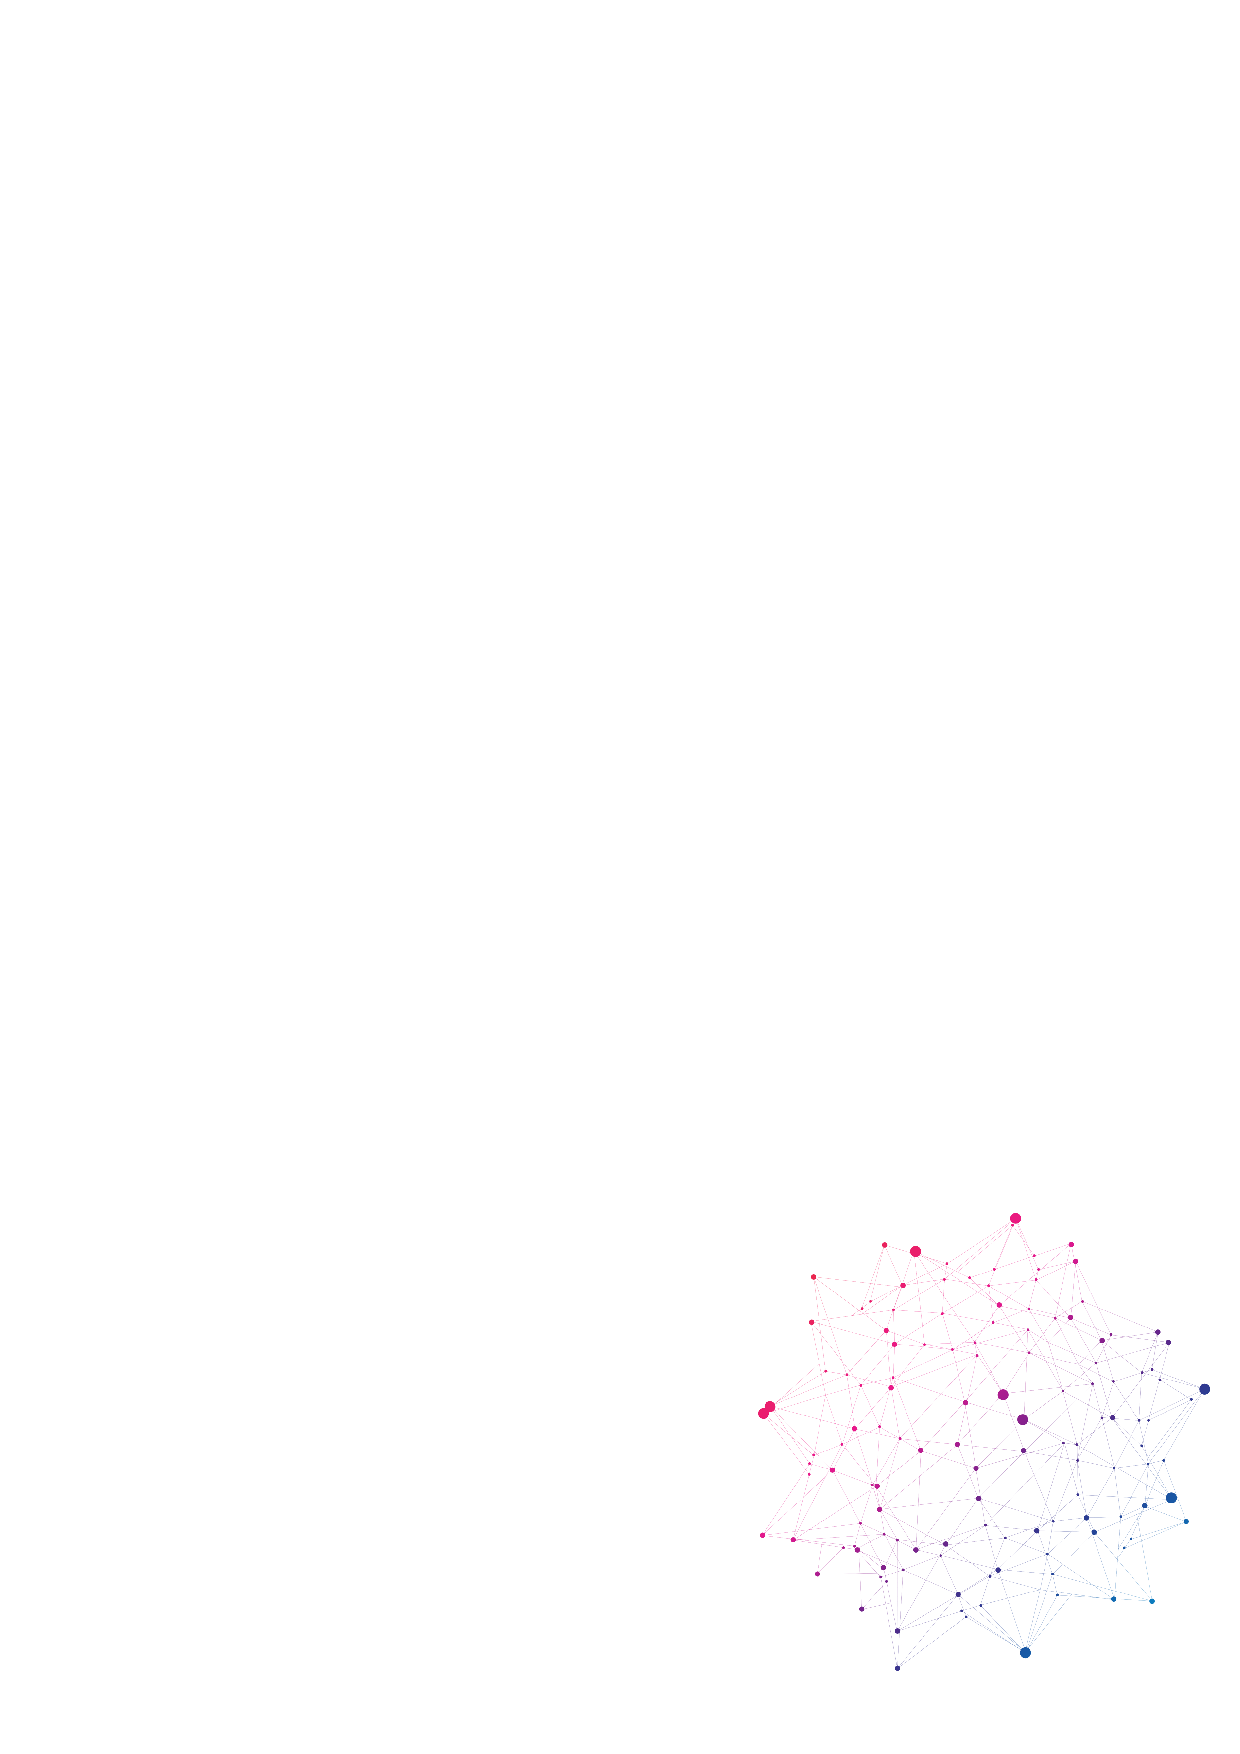
\includegraphics[width=\paperwidth]{Images/background.pdf}}
    \vspace*{1.2cm}
    \hspace*{1cm}{\Large Thank you!}\\
    \vspace*{0.6cm}
    \hspace*{1cm}{\Huge \alert{Any questions?}}
\end{frame}

\section*{Extra}

\begin{frame}{Prior ratio}

As a prior, we use an EPPF induced by the \alert{two-parameter Poisson-Dirichlet} process (Pitman-Yor process) from \cite{martinezNonparametricChangePoint2014}.
% TODO La formula tenetela in appendice (mi riferisco a slide 16) ma scrivetela giusta con la funzione indicatrice. 

Let $M$ and $p$ be the number of groups and nodes, respectively, and $n_{j},j=1,\ldots,M$ the cardinalities of the groups, $\theta$ and $\sigma$ are parameters.

\begin{equation*}
    P(\rho = \{n_1, \ldots, n_M\})
    =
    \frac{p!}{M!} \frac{ \prod_{i=1}^{M-1}{(\theta +i\sigma)} }{(\theta+1)_{(p-1)\uparrow}} \prod_{j=1}^{M}{\frac{(1-\sigma)_{(n_{j}-1)\uparrow}}{n_{j\uparrow}} }
\end{equation*}

Hence, in the split case, after simplifying common factors, the \alert{prior ratio} is:

\begin{equation*}
    \frac{f_{\rho}(\rho')}{f_{\rho}(\rho)}
    =
    \frac{1}{M}(\theta+M\sigma)\frac{(1-\sigma)_{(n_{s}'-1)\uparrow}(1-\sigma)_{(n_{s}'+1)\uparrow}}{(1-\sigma)_{(n_{s}-1)\uparrow}}\frac{n_{s}!}{n'_{s}!n'_{s+1}!}
\end{equation*}

\end{frame}

\begin{frame}{Likelihood ratio}

Suppose a split move.

The \alert{likelihood ratio}, after simplifying common factors, is:
% Anche S^star, decidete tra lui e il T.  TODO
{
    \footnotesize
    \begin{align*}
        & \frac{f_G(G \mid \rho^\prime)}{f_G(G \mid \rho)}=\left(\frac{1}{B(\alpha, \beta)}\right)^{M+1} \times \\
        & \frac{ \prod_{l=1}^{S-1} f_B(C_l^\prime, C_S^\prime) f_B(C_l^\prime, C_{S+1}^\prime) \cdot \prod_{m=S+2}^{M+1} f_B(C_S^\prime, C_m^\prime) f_B(C_{S+1}^\prime, C_m^\prime) \cdot f_B(C_S^\prime, C_{S+1}^\prime) f_B(C_S^\prime, C_S^\prime) f_B(C_{S+1}^\prime, C_{S+1}^\prime)}{\prod_{l=1}^{S-1} f_B(C_l, C_S) \prod_{m=S+1}^M f_B(C_S, C_m) \cdot f_B(C_S, C_S)} 
    \end{align*}
}

where

\[
    f_B(C_u, C_v) = B(\alpha+S_{uv},\beta+S^{\star}_{uv})
\]

and $S_{uv}$ is the sum of the edges between group $u$ and group $v$, and $S^{\star}_{uv}$ is the sum of non-edges.

\end{frame}

%\end{multicols}

% USE NOCITE TO ADD SOURCES TO THE BIBLIOGRAPHY WITHOUT SPECIFICALLY CITING THEM IN THE DOCUMENT
%\nocite{zhixiong_modelling_2015}
%\nocite{*}

% \begin{minted}{R}
% fib <- function(n) {
%   if (n < 2)
%     n
%   else
%     fib(n - 1) + fib(n - 2)
% }
% fib(10) # => 55
% \end{minted}
% 
% \begin{minted}{R}
% # Creating a Graph
% attach(mtcars)
% plot(wt, mpg)
% abline(lm(mpg~wt))
% title("Regression of MPG on Weight")
% \end{minted}

\nocite{*}
\printbibliography

\end{document}
